\documentclass[12pt,a4paper]{article}
\usepackage{parskip}
\usepackage{pdfpages}
\usepackage{hyperref}
\usepackage{amsmath}
\usepackage{pgfplots}
\usepackage{caption}
\usepackage{subcaption}
\usepackage{listings}

\usepackage[margin=.6in]{geometry}

\usepgfplotslibrary{fillbetween}

\definecolor{mygreen}{rgb}{0,0.6,0}
\definecolor{mygray}{rgb}{0.5,0.5,0.5}
\definecolor{mymauve}{rgb}{0.58,0,0.82}

\lstset{ %
  backgroundcolor=\color{white},   % choose the background color
  basicstyle=\footnotesize,        % size of fonts used for the code
  breaklines=true,                 % automatic line breaking only at whitespace
  captionpos=b,                    % sets the caption-position to bottom
  commentstyle=\color{mygreen},    % comment style
  escapeinside={\%*}{*)},          % if you want to add LaTeX within your code
  keywordstyle=\color{blue},       % keyword style
  stringstyle=\color{mymauve},     % string literal style
}

\begin{document}

\title{ECE 457B Assignment 2}
\date{March 7th, 2017}
\author{Lariesa Janecka, 20460089}
\maketitle

\section*{Question 1}
\label{sec:question_1}

\begin{figure}[h!]
\captionsetup[subfigure]{font=footnotesize}
\centering
\resizebox {3.5in} {!} {
\subcaptionbox*{$\mu_{A_1}$}[.5\textwidth]{%
\begin{tikzpicture}[
  declare function={
    func(\x)= (\x<2) * (0)   +
     and(\x>=2, \x<=5) * ((\x-2)/3)     +
     and(\x>5,  \x<=8) * ((8-x)/3) +
                (\x>8) * (0);
  }
]
\begin{axis}[
  axis x line=middle, axis y line=middle,
  ymin=0, ymax=1.33, ytick={0,0.33,0.66,1},
  xmin=0, xmax=12, xtick={0,...,12}, xlabel=$x$,
]
\pgfplotsinvokeforeach{4}{
  \draw[dashed] ({rel axis cs: 0,0} -| {axis cs: #1, 0}) -- ({rel axis cs: 0,1} -| {axis cs: #1, 0});}
\addplot[blue, domain=0:12]{func(x)};
\node[label={180:{0.66}},circle,fill,inner sep=2pt] at (axis cs:4,0.66) {};
\end{axis}
\end{tikzpicture}}}
\resizebox {3.5in} {!} {
\subcaptionbox*{$\mu_{B_1}$}[.5\textwidth]{%
\begin{tikzpicture}[
  declare function={
    func(\x)= (\x<5) * (0)   +
     and(\x>=5, \x<=8) * ((\x-5)/3)     +
     and(\x>8,  \x<=11) * ((11-x)/3) +
                (\x>11) * (0);
  }
]
\begin{axis}[
  axis x line=middle, axis y line=middle,
  ymin=0, ymax=1.33, ytick={0,0.33,0.66,1},
  xmin=0, xmax=12, xtick={0,...,12}, xlabel=$y$,
]
\pgfplotsinvokeforeach{8}{
  \draw[dashed] ({rel axis cs: 0,0} -| {axis cs: #1, 0}) -- ({rel axis cs: 0,1} -| {axis cs: #1, 0});}
\addplot[blue, domain=0:12]{func(x)};
\node[label={180:{1}},circle,fill,inner sep=2pt] at (axis cs:8,1) {};
\end{axis}
\end{tikzpicture}}}
\end{figure}
The strength of these two rules is 0.66 and the resulting and the cut on $\mu_{C_1}$ will occur at the max, which is 1.

\begin{figure}[h!]
\centering
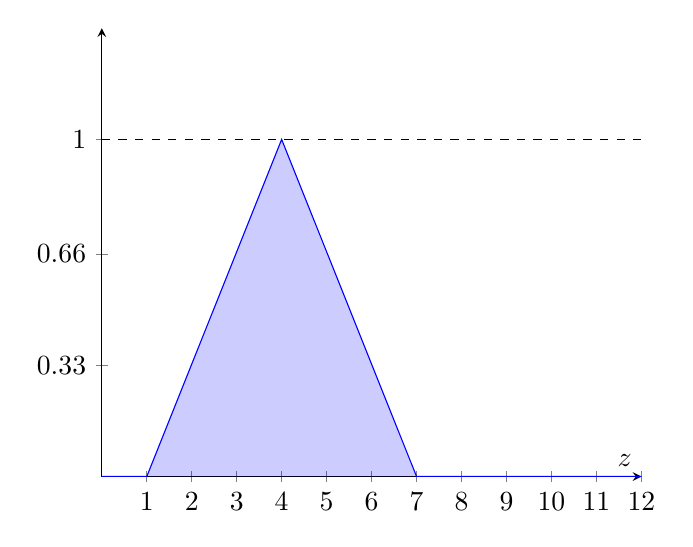
\begin{tikzpicture}[
  declare function={
    func(\x)= (\x<1) * (0)   +
     and(\x>=1, \x<=4) * ((\x-1)/3)     +
     and(\x>4,  \x<=7) * ((7-x)/3) +
                (\x>7) * (0);
  }
]
\begin{axis}[
  axis x line=middle, axis y line=middle,
  ymin=0, ymax=1.33, ytick={0,0.33,0.66,1},
  xmin=0, xmax=12, xtick={0,...,12}, xlabel=$z$,
]
\addplot[blue, domain=0:12, fill=blue, fill opacity=0.2]{func(x)};
  \draw[dashed] ({axis cs: 0, 1}) -- ({axis cs: 12, 1});
\end{axis}
\end{tikzpicture}
\caption*{$\mu_{C_1}$}
\end{figure}

\newpage


\begin{figure}[h!]
\captionsetup[subfigure]{font=footnotesize}
\centering
\resizebox {3.5in} {!} {
\subcaptionbox*{$\mu_{A_2}$}[.5\textwidth]{%
\begin{tikzpicture}[
  declare function={
    func(\x)= (\x<3) * (0)   +
     and(\x>=3, \x<=6) * ((\x-3)/3)     +
     and(\x>6,  \x<=9) * ((9-x)/3) +
                (\x>9) * (0);
  }
]
\begin{axis}[
  axis x line=middle, axis y line=middle,
  ymin=0, ymax=1.33, ytick={0,0.33,0.66,1},
  xmin=0, xmax=12, xtick={0,...,12}, xlabel=$x$,
]
\pgfplotsinvokeforeach{4}{
  \draw[dashed] ({rel axis cs: 0,0} -| {axis cs: #1, 0}) -- ({rel axis cs: 0,1} -| {axis cs: #1, 0});}
\addplot[blue, domain=0:12]{func(x)};
\node[label={180:{0.33}},circle,fill,inner sep=2pt] at (axis cs:4,0.33) {};
\end{axis}
\end{tikzpicture}}}
\resizebox {3.5in} {!} {
\subcaptionbox*{$\mu_{B_2}$}[.5\textwidth]{%
\begin{tikzpicture}[
  declare function={
    func(\x)= (\x<4) * (0)   +
     and(\x>=4, \x<=7) * ((\x-4)/3)     +
     and(\x>7,  \x<=10) * ((10-x)/3) +
                (\x>10) * (0);
  }
]
\begin{axis}[
  axis x line=middle, axis y line=middle,
  ymin=0, ymax=1.33, ytick={0,0.33,0.66,1},
  xmin=0, xmax=12, xtick={0,...,12}, xlabel=$y$,
]
\pgfplotsinvokeforeach{8}{
  \draw[dashed] ({rel axis cs: 0,0} -| {axis cs: #1, 0}) -- ({rel axis cs: 0,1} -| {axis cs: #1, 0});}
\addplot[blue, domain=0:12]{func(x)};
\node[label={360:{0.66}},circle,fill,inner sep=2pt] at (axis cs:8,0.66) {};
\end{axis}
\end{tikzpicture}}}
\end{figure}
The strength of these two rules is 0.33 and the resulting and the cut on $\mu_{C_1}$ will occur at the max, which is 0.66.

\begin{figure}[h!]
\centering
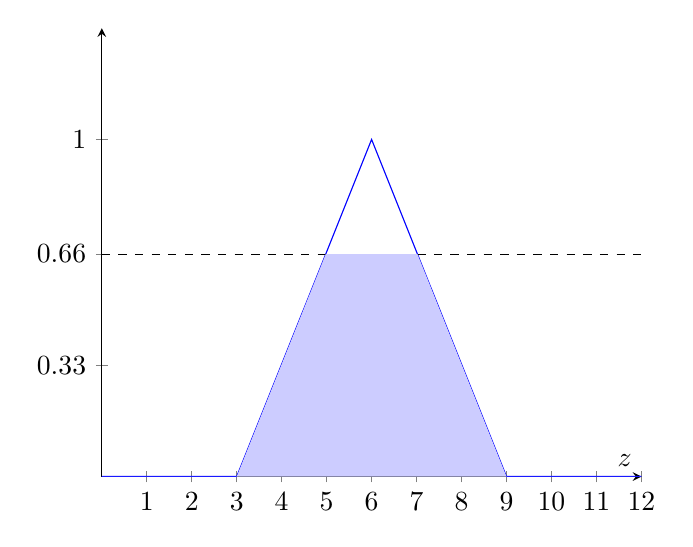
\begin{tikzpicture}[
  declare function={
    func(\x)= (\x<3) * (0)   +
     and(\x>=3, \x<=6) * ((\x-3)/3)     +
     and(\x>6,  \x<=9) * ((9-x)/3) +
                (\x>9) * (0);
  }
]
\begin{axis}[
  axis x line=middle, axis y line=middle,
  ymin=0, ymax=1.33, ytick={0,0.33,0.66,1},
  xmin=0, xmax=12, xtick={0,...,12}, xlabel=$z$,
]
\addplot[name path=f, blue, domain=0:12]{func(x)};
\addplot[name path=cut, black, dashed, domain=0:12]{0.66};

\path[name path=axis] ({axis cs: 0, 0}) -- ({axis cs: 12, 0});

\fill[blue!20!white,intersection segments={of=f and cut,sequence={A0 -- B1 -- A2}}]
    -- (axis cs:12,\pgfkeysvalueof{/pgfplots/ymin})
    -- (axis cs:0,\pgfkeysvalueof{/pgfplots/ymin})
    -- cycle
;
\end{axis}
\end{tikzpicture}
\caption*{$\mu_{C_2}$}
\end{figure}

\begin{figure}[h!]
\centering
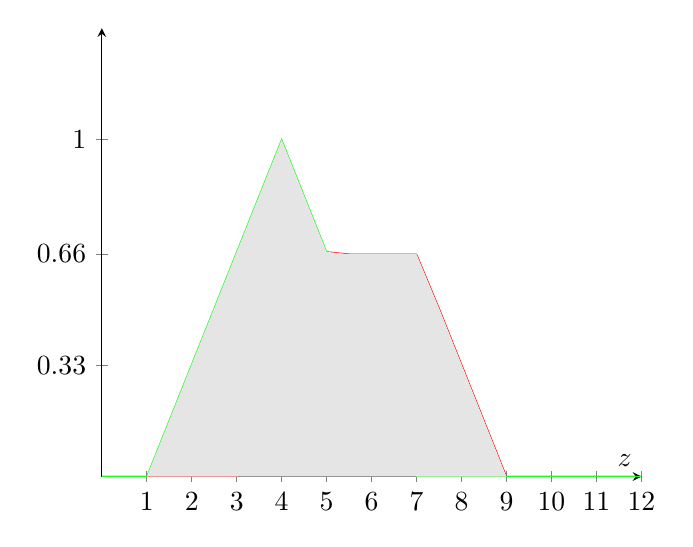
\begin{tikzpicture}[
  declare function={
    func1(\x)= (\x<3) * (0)   +
     and(\x>=3, \x<=5) * ((\x-3)/3)     +
     and(\x>5,  \x<=7) * (0.66) +
     and(\x>7,  \x<=9) * ((9-x)/3) +
                (\x>9) * (0);
  },
  declare function={
    func2(\x)= (\x<1) * (0)   +
     and(\x>=1, \x<=4) * ((\x-1)/3)     +
     and(\x>4,  \x<=7) * ((7-x)/3) +
                (\x>7) * (0);
  }
]
\begin{axis}[
  axis x line=middle, axis y line=middle,
  ymin=0, ymax=1.33, ytick={0,0.33,0.66,1},
  xmin=0, xmax=12, xtick={0,...,12}, xlabel=$z$,
]
\addplot[name path=f1, red, domain=0:12]{func1(x)};
\addplot[name path=f2, green, domain=0:12]{func2(x)};

\path[name path=axis] ({axis cs: 0, 0}) -- ({axis cs: 12, 0});

\fill[black!10!white,intersection segments={of=f1 and f2,sequence={A0 -- B1 -- A2}}]
    -- (axis cs:12,\pgfkeysvalueof{/pgfplots/ymin})
    -- (axis cs:0,\pgfkeysvalueof{/pgfplots/ymin})
    -- cycle
;
\end{axis}
\end{tikzpicture}
\caption*{output}
\end{figure}

In this instance we have only one maximum at 4 so the mean of maxima is 4, giving us the defuzzified output at $t_1$.

When calculating for the centroid of area a slightly different answer occurs.

\begin{align*}
	c &= \frac{\int c\mu_c(c)\delta c}{\int \mu_c(c)\delta c}\\
		&= \frac{\int_1^5 \frac{x-1}{3}x\delta x + \int_5^70.66x\delta x + \int_7^9 \frac{9-x}{3}x\delta x}
			{\int_1^5 \frac{x-1}{3}\delta x + \int_5^70.66\delta x + \int_7^9 \frac{9-x}{3}\delta x}\\
		&= \frac{22.8089}{4.6533}\\
		&= 4.9016
\end{align*}

The centroid of area is slightly higher because the mean of maxima disregards the values outside of its single peak. This is also why the centroid of area returns a more accurate result.

\section*{Question 2}
\label{sec:question_2}
\subsection*{a)}
\label{sub:a_}
\subsubsection*{i)}
\label{ssub:i_}
Classical:

\begin{tabular}{c | c c c c c c c}
f\textbackslash K & $1e+3$ & $1e+4$ & $1e+5$ & $5e+5$ & $1e+6$ & $5e+6$ & $1e+7$\\
\hline
100  & 1  & 0.8  & 0.5  & 0.2  & 0  & 0.2  & 0.8 \\
200  & 1  & 0.8  & 0.5  & 0.2  & 0  & 0.2  & 0.8 \\
500  & 1  & 0.8  & 0.5  & 0.2  & 0.2  & 0.2  & 0.8 \\
800  & 1  & 0.8  & 0.5  & 0.5  & 0.5  & 0.5  & 0.8 \\
1000 & 1  & 0.8  & 0.5  & 0.8  & 1  & 0.8  & 0.8 \\
2000 & 1  & 0.8  & 0.5  & 0.8  & 0.8  & 0.8  & 0.8 \\
5000 & 1  & 0.8  & 0.5  & 0.2  & 0.2  & 0.2  & 0.8 \\
\end{tabular}

\subsubsection*{ii)}
\label{ssub:ii_}
Mamdani:

\begin{tabular}{c | c c c c c c c}
f\textbackslash K & $1e+3$ & $1e+4$ & $1e+5$ & $5e+5$ & $1e+6$ & $5e+6$ & $1e+7$\\
\hline
100  & 0  & 0  & 0  & 0  & 0  & 0  & 0 \\
200  & 0  & 0  & 0  & 0  & 0  & 0  & 0 \\
500  & 0  & 0.2  & 0.2  & 0.2  & 0.2  & 0.2  & 0.2 \\
800  & 0  & 0.2  & 0.5  & 0.5  & 0.5  & 0.5  & 0.2 \\
1000 & 0  & 0.2  & 0.5  & 0.8  & 1  & 0.8  & 0.2 \\
2000 & 0  & 0.2  & 0.5  & 0.8  & 0.8  & 0.8  & 0.2 \\
5000 & 0  & 0.2  & 0.2  & 0.2  & 0.2  & 0.2  & 0.2 \\
\end{tabular}

\subsubsection*{iii)}
\label{ssub:iii_}
Product:

\begin{tabular}{c | c c c c c c c}
f\textbackslash K & $1e+3$ & $1e+4$ & $1e+5$ & $5e+5$ & $1e+6$ & $5e+6$ & $1e+7$\\
\hline
100   & 0  & 0.0  & 0.0  & 0.0  & 0  & 0.0  & 0.0 \\
200   & 0  & 0.0  & 0.0  & 0.0  & 0  & 0.0  & 0.0 \\
500 & 0.0  & 0.04  & 0.1  & 0.16  & 0.2  & 0.16  & 0.04 \\
800 & 0.0  & 0.1  & 0.25  & 0.4  & 0.5  & 0.4  & 0.1 \\
1000   & 0  & 0.2  & 0.5  & 0.8  & 1  & 0.8  & 0.2 \\
2000 & 0.0  & 0.16  & 0.4  & 0.64  & 0.8  & 0.64  & 0.16 \\
5000 & 0.0  & 0.04  & 0.1  & 0.16  & 0.2  & 0.16  & 0.04 \\
\end{tabular}

\subsection*{b)}
\label{sub:b_}
\begin{align*}
	R &=\begin{bmatrix}
		1  & 0.8  & 0.5  & 0.2  & 0  & 0.2  & 0.8 \\
		1  & 0.8  & 0.5  & 0.2  & 0  & 0.2  & 0.8 \\
		1  & 0.8  & 0.5  & 0.2  & 0.2  & 0.2  & 0.8 \\
		1  & 0.8  & 0.5  & 0.5  & 0.5  & 0.5  & 0.8 \\
		1  & 0.8  & 0.5  & 0.8  & 1  & 0.8  & 0.8 \\
		1  & 0.8  & 0.5  & 0.8  & 0.8  & 0.8  & 0.8 \\
		1  & 0.8  & 0.5  & 0.2  & 0.2  & 0.2  & 0.8 \\
	\end{bmatrix}\\
	K' &=\begin{bmatrix}
		0\\
		0.8\\
		0.2\\
	\end{bmatrix}\\
	f_1 &= R \circ K'\\
		&= \max_{rows} \left(\min_{cols} \left(K', R\right)\right)\\
		&= \max_{cols} \left(\min_{cols} \left(
		\begin{bmatrix}
			0\\
			0.8\\
			0.2\\
		\end{bmatrix},
	\begin{bmatrix}
		1  & 0.8  & 0.5  & 0.2  & 0  & 0.2  & 0.8 \\
		1  & 0.8  & 0.5  & 0.2  & 0  & 0.2  & 0.8 \\
		1  & 0.8  & 0.5  & 0.2  & 0.2  & 0.2  & 0.8 \\
		1  & 0.8  & 0.5  & 0.5  & 0.5  & 0.5  & 0.8 \\
		1  & 0.8  & 0.5  & 0.8  & 1  & 0.8  & 0.8 \\
		1  & 0.8  & 0.5  & 0.8  & 0.8  & 0.8  & 0.8 \\
		1  & 0.8  & 0.5  & 0.2  & 0.2  & 0.2  & 0.8 \\
	\end{bmatrix}
		\right)
		\right)\\
	&= \max_{cols} \left(
	\begin{bmatrix}
		0 & 0 & 0 & 0 & 0 & 0 & 0\\
		0.8 & 0.8 & 0.5 & 0.2 & 0 & 0.2 & 0.8\\
		0.2 & 0.2 & 0.2 & 0.2 & 0.2 & 0.2 & 0.2\\
	\end{bmatrix}
		\right)\\
	&= \begin{bmatrix}
		0.8 & 0.8 & 0.5 & 0.2 & 0.2 & 0.2 & 0.8\\
		\end{bmatrix}\\
\end{align*}

\section*{Question 3}
\label{sec:question_3}
\begin{align*}
	T_{300} &= \left\{\frac{0}{LW} + \frac{1}{HG}\right\} \\
	M_{800} &= \left\{\frac{0}{SM} + \frac{1}{LG}\right\} \\
	P_{1.3} &= \left\{\frac{0.2}{FR} + \frac{0.8}{NR}\right\} \\
\end{align*}

Rule 1: If $T$ is $LW$ and $P$ is $FR$ then $F$ is $IN$: $\left \{ \frac{0}{LW} + \frac{0.2}{FR}\right\} = \frac{0}{IN}$

Rule 2: If $T$ is $HG$ then $F$ is $RD$: $\left \{ \frac{1}{HG} \right \} = \frac{1}{RD}$

Rule 3: If $M$ is $SM$ and $P$ is $NR$ then $F$ is $MN$: $\left \{ \frac{0}{SM} + \frac{0.8}{NR} \right \} = \frac{0}{MN}$

Rule 4: If $M$ is $LG$ and $P$ is $FR$ then $F$ is $IN$: $\left \{ \frac{1}{LG} + \frac{0.2}{FR} \right \} = \frac{0.2}{IN}$

Rule 5: If $P$ is $NR$ then $F$ is $RD$: $\left \{ \frac{0.8}{NR} \right \} = \frac{0.8}{RD}$

Then $F = \left \{ \frac{1}{RD} + \frac{0.2}{IN}\right \}$

When these is applied you get a membership function of:
\begin{align}
	f &= \begin{cases}
		0.8, \texttt{ if } x \leq 5.4\\
		(5-x)/2, \texttt{ if } 5.4 < x \leq 7\\
		0, \texttt{ if } 7 < x \leq 12\\
		(x-12)/2, \texttt{ if } 12 < x \leq 12.4\\
		0.2, \texttt{ if } x < 12\\
	\end{cases}
\end{align}

Applying the centroid of area gives a value of 6.23

This value seems to make sense as it falls roughly in the middle. Since the temperature is very high you might want to reduce the fuel rate, but the mass is very large so you might want to increase the temperature.


\section*{Question 4}
\label{sec:question_4}
\subsection*{a)}
\label{sub:a_}

Input 1:
\begin{align*}
	r &= \sum_i w_i x_i\\
	&= (1)(1) + (-2)(-1) + (0)(0) + (-1)(0.5)\\
	&= 2.5\\
	\Delta w &= \eta(t_1 - r)x_1\\
	&= 0.1(-1-2.5)\begin{bmatrix}
		1 & -2 & 0 & -1
	\end{bmatrix}\\
	&= \begin{bmatrix}
		-0.35 & 0.7 & 0 & -0.35
	\end{bmatrix}\\
	w^{(2)} &= w^{(1)} - \Delta w\\
	&=
	\begin{bmatrix}
		1 & -1 & 0.5 & -1
	\end{bmatrix} -
	\begin{bmatrix}
		-0.35 & 0.7 & 0 & -0.35
	\end{bmatrix}\\
	&=
	\begin{bmatrix}
		1.35 & -1.7 & 0.5 & 1.35
	\end{bmatrix}\\
\end{align*}
Input 2:
\begin{align*}
	r &= (1.35)(0) + (-1.7)(1.5) + (0.5)(-0.5) + (1.35)(-1)\\
	&= -4.15\\
	\Delta w &= 0.1(-1+4.15)\begin{bmatrix}
		0 & 1.5 & -0.5 & -1
	\end{bmatrix}\\
	&= \begin{bmatrix}
		0 & 0.47 & -0.16 & -0.315
	\end{bmatrix}\\
	w^{(3)} &=
	\begin{bmatrix}
		1.35 & -1.7 & 0.5 & 1.35
	\end{bmatrix} -
	\begin{bmatrix}
		0 & 0.47 & -0.16 & -0.315
	\end{bmatrix}\\
	&=
	\begin{bmatrix}
		1.35 & -2.17 & 0.66 & 1.665
	\end{bmatrix}\\
\end{align*}
Input 3:
\begin{align*}
	r &= (1.35)(-1) + (-2.7)(1) + (0.66)(0.5) + (1.665)(-1)\\
	&= −5.385\\
	\Delta w &= 0.1(1+5.385)\begin{bmatrix}
		-1 & 1 & 0.5 & -1
	\end{bmatrix}\\
	&= \begin{bmatrix}
		-0.6385 & 0.6385 & 0.31925 & -0.6385
	\end{bmatrix}\\
	w^{(4)} &=
	\begin{bmatrix}
		1.35 & -2.17 & 0.66 & 1.665
	\end{bmatrix} -
\begin{bmatrix}
		-0.6385 & 0.6385 & 0.31925 & -0.6385
	\end{bmatrix}\\
	&=
	\begin{bmatrix}
		1.9885 & −3.3385 & 0.34075 & 2.3035
	\end{bmatrix}\\
\end{align*}

\subsection*{b)}
\label{sub:b_}
Code is also attached in q4.py

\begin{lstlisting}[language=python]
# Training data
x1 = [1, -2, 0, -1]
x2 = 0, 1.5, -0.5, -1
x3 = [-1, 1, 0.5, -1]
inputs = [x1, x2, x3]
# Labels for training data
t1 = -1
t2 = -1
t3 = 1
targets = [t1, t2, t3]
# Initial weights
weights = [1, -1, 0, 0.5]
# Learning rate
n = 0.1
# Maximum number of iterations
maxIterations = 50
# Thresholds for determining if a steady state has been achieved
threshold = 0.1

def calcR(i):
    r = 0
    for j in range(0, len(inputs[i])):
            r += inputs[i][j] * weights[j]
    return r

iters = 0
while iters < maxIterations: # loop for each epoch
    output = 0
    isSteady = True
    for i in range(0, len(inputs)): #loop for each piece of training data
        r = calcR(i)
        for data in range(0, len(weights)):
            # Calculate delta
            delta =  n * (targets[i] - r) * inputs[i][data]
            # Check if delta is close enough to 0
            isSteady = isSteady and (abs(delta) < threshold)
            # Update weights
            weights[data] = weights[data] + delta
    if isSteady: # stop looping if steady state has been achieved
        break
    iters += 1
if iters == maxIterations - 1:
    print 'Did not converge'
else:
    print 'Converged in {0} epochs'.format(iters)
    print weights
\end{lstlisting}

The output for this was that the training data was linearly separable in 6 epochs and weights $\begin{bmatrix}
	-0.36 & 0.17 & 0.68 & 0.34
\end{bmatrix}$ (rounded to 2 digits).

\subsection*{c)}
\label{sub:c_}
\begin{align*}
	u &= \begin{bmatrix}
		-1 & -1 & 0 & 0.5
	\end{bmatrix}\\
	w &= \begin{bmatrix}
		-0.36 & 0.17 & 0.68 & 0.34
	\end{bmatrix}\\
	r &= (-1)(-0.6) + (-1)(0.17) + (0)(0.68) + (0.5)(0.34)\\
	&= 0.6\\
	signum(r) &= 1\\
\end{align*}

So u belongs in class C1.

\section*{Question 5}
\label{sec:question_5}
For brevity's sake we will abbreviate:
\begin{align}
	r^{(k)} &= \sum_i w_ix_i^{(k)}+\theta
\end{align}

This makes the new error function:
\begin{align*}
	E(w) &= \sum_i \left( t^{(k)} - S(r^{(k)}) \right)^2\\
	&= \sum_i \left( t^{(k)} - \frac{1}{1+e^{r^{(k)}}} \right)^2\\
\end{align*}

\begin{align*}
	\nabla_w E(w) &= \frac{\delta E(w)}{\delta w}\\
	&= \frac{\delta \left( t^{(k)} - \frac{1}{1+e^{r^{(k)}}} \right)^2}{\delta w}\\
	&= \frac{\delta \left( t^{(k)} - \frac{1}{1+e^{r^{(k)}}} \right)^2}{\delta r^{(k)}} \frac{\delta r^{(k)}}{\delta w}\\
	&= 2\left( t^{(k)} - \frac{1}{1+e^{r^{(k)}}} \right) \frac{\delta \left( t^{(k)} - \frac{1}{1+e^{r^{(k)}}} \right)}{\delta r^{(k)}} \frac{\delta r^{(k)}}{\delta w}\\
	&= 2\left( t^{(k)} - \frac{1}{1+e^{r^{(k)}}} \right) \left ( 0 - \frac{\delta \left(\frac{1}{1+e^{r^{(k)}}} \right)}{\delta r^{(k)}} \right) \frac{\delta r^{(k)}}{\delta w}\\
	&= 2\left( t^{(k)} - \frac{1}{1+e^{r^{(k)}}} \right) \left (\frac{e^{r^{(k)}}}{(1+e^{r^{(k)}})^2} \right) \frac{\delta r^{(k)}}{\delta w}\\
	&= 2\left( t^{(k)} - \frac{1}{1+e^{r^{(k)}}} \right) \left (\frac{e^{r^{(k)}}}{(1+e^{r^{(k)}})^2} \right)x_i\\
	\Delta w &= -\eta \nabla_wE(w)\\
	&= -\eta\left( t^{(k)} - \frac{1}{1+e^{r^{(k)}}} \right) \left (\frac{e^{r^{(k)}}}{(1+e^{r^{(k)}})^2} \right)x_i\\
\end{align*}



























\end{document}
